\documentclass[11pt]{article}

\usepackage[margin=1in]{geometry}
\usepackage[T1]{fontenc}
\usepackage[utf8]{inputenc}
\usepackage{lmodern}
\usepackage{booktabs}
\usepackage{amsmath}
\usepackage{enumitem}
\usepackage{graphicx}
\usepackage{hyperref}
\usepackage{xcolor}

\hypersetup{
  colorlinks=true,
  linkcolor=blue,
  urlcolor=blue,
  citecolor=blue,
  pdftitle={Interpretable Linear Reinforcement Learning for Orbit Chase}
}

\newcommand{\todo}[1]{\textcolor{red}{[TODO: #1]}}

\title{When Is Linear On-Policy Control Enough?\\
An Empirical Study of True Online Sarsa($\lambda$) in a Procedurally Generated 2D Pursuit-and-Collection Game}
\author{\todo{Author name}\\\todo{Institution or course}}
\date{\today}

\begin{document}
\maketitle

\begin{abstract}
This paper studies whether an interpretable linear reinforcement-learning
controller can solve a structured 2D pursuit-and-collection task without a
neural network. I introduce Orbit Chase, a deterministic continuous arena in
which a player must collect 32 pellets while avoiding a fixed greedy enemy,
static obstacle bars, and a 60-second time limit. The agent receives a
130-dimensional observation vector and an eight-action collision-aware mask.
I train a linear True Online Sarsa($\lambda$) agent with sparse hashed tile
coding, engineered relative features, and masked epsilon-greedy control.
One frozen policy trained for 8,000 episodes cleared 96 of 100 episodes on a
documented evaluation seed range and 8,970 of 10,000 episodes in a broader
post-training sweep of unseen procedural arenas. The result substantially
exceeds three non-learning baselines. The paper argues that a linear value
function can perform strongly when the environment supplies structured numeric
state, the feature map preserves relevant geometry, and action masking removes
unsafe moves. The evidence applies to this fixed game distribution and one
training run; it does not establish robustness across training seeds,
opponents, or arbitrary 2D games.
\end{abstract}

\section{Introduction}

Deep reinforcement learning is often the default choice for game-control
problems. That choice is less compelling when an environment exposes compact,
structured numeric state rather than pixels. Linear value-function methods
remain useful in that setting because they are inspectable, inexpensive, and
make the relationship between state representation and control performance
visible \cite{sutton-barto-2018,van-seijen-2016}.

This paper asks the following question:

\begin{quote}
Can an interpretable linear on-policy reinforcement-learning agent clear a
procedurally generated 2D pursuit-and-collection game more effectively than
hand-coded baselines?
\end{quote}

The study evaluates a linear True Online Sarsa($\lambda$) controller in Orbit
Chase. Orbit Chase is a continuous top-down arena, not a grid world. Its state
is also not a collection of 130 discrete states; it is represented by a
130-dimensional observation vector whose positions, velocities, timers, and
procedural layouts create a large continuous and combinatorial state space.

The contributions are:

\begin{enumerate}[leftmargin=*]
  \item a deterministic player-control environment with a Python Gymnasium
  interface and matching TypeScript game simulation;
  \item a sparse, engineered tile-coded feature representation for linear True
  Online Sarsa($\lambda$);
  \item reproducible seeded training, checkpointing, baseline evaluation, and
  Python--TypeScript rule-parity tests; and
  \item an empirical comparison showing high greedy clear rates for one frozen
  linear policy under the specified procedural-arena distribution.
\end{enumerate}

\section{Orbit Chase as a Markov Decision Process}

\subsection{Game dynamics}

The yellow player wins by collecting all 32 pellets within 60 seconds. A red
enemy follows a deterministic greedy pursuit rule and captures the player on
contact. The circular arena contains a central core, two static procedural
obstacle bars, and three Surge Orbs. A collected Surge Orb gives the player a
four-second speed advantage.

Physics advances in fixed 10 ms ticks. The player selects one of eight
directions every 100 ms and holds that direction for ten physics ticks. The
enemy selects a collision-safe pursuit direction every 280 ms. A fixed enemy
turns the task into a single-agent MDP: the enemy belongs to the transition
dynamics rather than acting as a second learning agent.

\subsection{Observation and actions}

Table~\ref{tab:observation} describes the player observation. Coordinates are
normalized around the arena center. The action mask is returned beside the
130-value observation; it identifies directions that can complete the next
100 ms movement interval without colliding with the boundary, core, or a bar.
The mask simulation accounts for Surge expiry and Orb pickups during the
interval.

\begin{table}[ht]
\centering
\caption{Fixed-order player observation.}
\label{tab:observation}
\begin{tabular}{lr}
\toprule
Feature group & Values \\
\midrule
Player position, velocity, and Surge fraction & 5 \\
Enemy position, heading, and decision-clock fraction & 11 \\
Two obstacle-bar endpoints & 8 \\
32 pellet positions and active flags & 96 \\
Three Orb positions and active flags & 9 \\
Remaining-time fraction & 1 \\
\midrule
Total observation size & 130 \\
Action-mask size & 8 \\
\bottomrule
\end{tabular}
\end{table}

The actions follow this fixed order:
\texttt{up}, \texttt{up-right}, \texttt{right}, \texttt{down-right},
\texttt{down}, \texttt{down-left}, \texttt{left}, and \texttt{up-left}.

\subsection{Reward and terminal conditions}

The reward combines progress toward clearing the arena with pressure to avoid
capture and avoid stalling:

\begin{table}[ht]
\centering
\caption{Reward schedule per player decision.}
\label{tab:rewards}
\begin{tabular}{lr}
\toprule
Event & Reward \\
\midrule
Clear all pellets & +100 \\
Collect one pellet & +3 \\
Collect one Surge Orb & +10 \\
Capture & -100 \\
Timeout & -30 \\
Each decision & -0.01 \\
\bottomrule
\end{tabular}
\end{table}

Capture takes precedence over a simultaneous clear when determining the
terminal outcome. Pellet and Orb rewards still accrue on the transition where
they are collected. Clear rate, rather than survival time, is the primary
metric because a timeout without collecting all pellets is not success.

\section{Method}

\subsection{Linear True Online Sarsa($\lambda$)}

The agent estimates one action value for each direction:

\begin{equation}
  Q(s,a) = w_a^\top \phi(s),
\end{equation}

where $\phi(s)$ is a sparse feature vector and $w_a$ is the weight vector for
action $a$. During training, the agent uses masked epsilon-greedy action
selection. Exploration samples uniformly from valid actions; greedy ties are
randomized during training. Evaluation freezes the weight matrix and selects
the lowest-index action among tied valid values.

The update uses the True Online Sarsa($\lambda$) formulation with sparse Dutch
eligibility traces. Nonterminal transitions bootstrap from the value of the
next action selected by the behavior policy. Capture, clear, and timeout
transitions use zero bootstrap. True-online temporal-difference methods retain
the forward-view interpretation of trace methods while supporting online
updates \cite{van-seijen-2016}.

\begin{table}[ht]
\centering
\caption{Selected training configuration.}
\label{tab:hyperparameters}
\small
\begin{tabular}{lr}
\toprule
Hyperparameter & Value \\
\midrule
Algorithm & True Online Sarsa($\lambda$) \\
$\lambda$ & 0.5 \\
$\gamma$ & 0.995 \\
Effective step size & 0.1 \\
Per-update step size & $0.1 / \lVert x \rVert^2$ \\
Initial / final $\epsilon$ & 0.20 / 0.02 \\
$\epsilon$-decay horizon & 8,000 episodes \\
Hash-table capacity & 262,144 \\
Tile bins / tilings & 8 / 8 \\
\bottomrule
\end{tabular}
\end{table}

\subsection{Rationale for Hyperparameters and Audit Corrections}

The final values were chosen as a small, inspectable linear-control baseline,
then refined after implementation audits. They should not be presented as a
fully optimized configuration: the project did not complete a multi-seed
hyperparameter search or a final-checkpoint validation study. Their rationale
is as follows.

\paragraph{Trace parameter $\lambda = 0.5$.}
Eligibility traces assign some credit to actions that occurred before a reward
or terminal event. A value of $\lambda = 0$ gives one-step Sarsa, whereas a
value close to $1$ propagates credit across a long sequence of decisions. The
final run used $0.5$ to retain multi-step credit assignment without allowing
traces to dominate a long and changing pursuit trajectory. This choice followed
an earlier $\lambda = 0.90$ experiment that was halted before completion. The
current evidence supports $0.5$ as the configuration used for the reported
result; it does not prove that $0.5$ is optimal.

\paragraph{Discount factor $\gamma = 0.995$.}
One agent decision covers 100 ms. The clear reward may occur hundreds of
decisions after an early movement choice, so the controller needs a long
planning horizon. With $\gamma = 0.995$, a reward 100 decisions, or ten
seconds, in the future retains about $0.995^{100} \approx 0.61$ of its value.
This value gives pellet collection and eventual clearing influence over
near-future actions while retaining some preference for earlier reward.

\paragraph{Effective step size 0.1 and per-update normalization.}
The tile-coded state activates roughly 120--128 binary features at one
decision. A fixed per-feature step size would make the total update grow with
the number of active features. The final implementation therefore uses

\begin{equation}
  \alpha_t = \frac{0.1}{\lVert x_t \rVert^2}.
\end{equation}

For binary features, $\lVert x_t \rVert^2$ is approximately the number of
active features. This normalization keeps the aggregate first-update scale
near 0.1 rather than multiplying it by the feature count. An audit found that
the earlier step-size treatment did not apply this normalization correctly;
the project invalidated those earlier checkpoints and retrained from scratch.

\paragraph{Exploration schedule $\epsilon: 0.20 \rightarrow 0.02$.}
The initial value of 0.20 forces exploration among valid directions while the
value function is untrained. The final value of 0.02 preserves limited
exploration late in training. Epsilon decays over a fixed 8,000-episode
horizon, independent of how many episodes a diagnostic run requests. This
detail matters: an audit found that decaying epsilon over the requested run
length made a short 800-episode diagnostic follow a different learning problem
from the intended 8,000-episode experiment.

\paragraph{Tile coding and hash capacity.}
Eight tilings provide overlapping discretizations, so nearby continuous values
share some active features while distinct regions can still receive different
weights. Eight bins set the resolution within each normalized range. The
262,144-bucket hash table keeps the sparse representation practical while
reducing, rather than eliminating, feature-hash collisions. These values were
selected as a tractable representation for the 130-dimensional observation;
ablation studies remain necessary to measure their individual contribution.

\subsection{Feature representation}

The agent does not tile-code the raw 130-value vector as one joint space. It
uses sparse hashed tile features for player position and velocity,
enemy-relative position, enemy heading and clock, Surge and time state, the
four nearest active pellets, the three active Orbs, the nearest point on each
bar, and the action mask. Each feature group has a separate salt before
hashing. Modulo hashing can still cause collisions, but separate salts avoid
semantic aliasing before the final hash reduction.

The representation reduces irrelevant order dependence. Active pellets are
ranked by distance to the player, and bar endpoints are canonicalized and
sorted. This design retains nearby collection targets and obstacles while
keeping the feature vector sparse enough for a linear method.

\section{Experimental Protocol}

\subsection{Environment seeds and evaluation}

The experiment uses disjoint seed ranges for procedural environments. These
ranges are not equivalent to a supervised-learning data split: training
generates trajectories while the policy changes. The correct RL evaluation
procedure freezes the policy, sets exploration to zero, and measures complete
greedy rollouts on environment seeds that did not contribute training updates.

\begin{table}[ht]
\centering
\caption{Seed ranges used by the experiment.}
\label{tab:seeds}
\begin{tabular}{ll}
\toprule
Purpose & Seed range \\
\midrule
Training episodes & 0--7,999 \\
Planned validation environments & 8,000--8,999 \\
Documented evaluation slice & 10,000--10,099 \\
Broader post-training sweep & 10,000--19,999 \\
\bottomrule
\end{tabular}
\end{table}

The selected run used agent random seed 73 and trained for 8,000 episodes. It
made 2,519,641 decisions, produced 3,144 exploratory training clears, and
left 33,195 nonzero weights across the eight action rows. The training log
contains one configuration record and 8,000 episode records.

\subsection{Baselines and metrics}

The agent is compared with three non-learning policies: random-valid,
pellet-seeking, and enemy-evade. Evaluation reports clear, capture, and
timeout rates; mean pellets collected; mean shaped return; and mean time to
clear among successful episodes.

\section{Results}

\subsection{Greedy policy comparison}

Table~\ref{tab:baseline-results} compares greedy Sarsa evaluation with the
baselines on seeds 10,000--10,099. The linear agent cleared 96 of 100 episodes
and collected 31.56 pellets on average. Pellet seeking cleared 10 episodes;
the other two baselines did not clear an episode.

\begin{table}[ht]
\centering
\caption{Evaluation on seeds 10,000--10,099.}
\label{tab:baseline-results}
\begin{tabular}{lrrr}
\toprule
Policy & Clears & Clear rate & Mean pellets \\
\midrule
Random valid & 0 / 100 & 0\% & 2.10 \\
Pellet seeking & 10 / 100 & 10\% & 13.62 \\
Enemy evade & 0 / 100 & 0\% & 1.41 \\
Linear True Online Sarsa($\lambda$) & 96 / 100 & 96\% & 31.56 \\
\bottomrule
\end{tabular}
\end{table}

For the linear agent, the 100-episode evaluation recorded one capture, three
timeouts, mean return 213.423, and mean successful clear time 27.775 seconds.

\subsection{Broader post-training sweep}

The same frozen checkpoint was evaluated on 10,000 procedural seeds from
10,000 through 19,999. It cleared 8,970 episodes (89.7\%), recorded 499
captures and 531 timeouts, collected 31.2288 pellets on average, achieved mean
return 201.645, and cleared successful episodes in 27.526 seconds on average.

The 100-seed slice belongs to the larger sweep and was evaluated more than
once during development. Therefore, the 89.7\% figure is reported as a broad
post-training fixed-seed benchmark, not as an untouched one-shot final test.
Assuming the procedural seeds behave as independent samples, the descriptive
95\% Wilson interval for 8,970 clears in 10,000 episodes is approximately
89.1\%--90.3\%. This interval describes variation across sampled environment
seeds, not variation across independently trained agents.

\subsection{Learning curve}

Exploratory training clear rate rose from 2.3\% during episodes 0--999 to
80.7\% during episodes 7,000--7,999. Because epsilon remained nonzero during
training, this curve shows learning progress but does not replace frozen greedy
evaluation. Figure~\ref{fig:sarsa-learning-curve} reports clear rate, mean
pellets collected, and mean return for each 1{,}000-episode block.

\begin{figure}[ht]
  \centering
  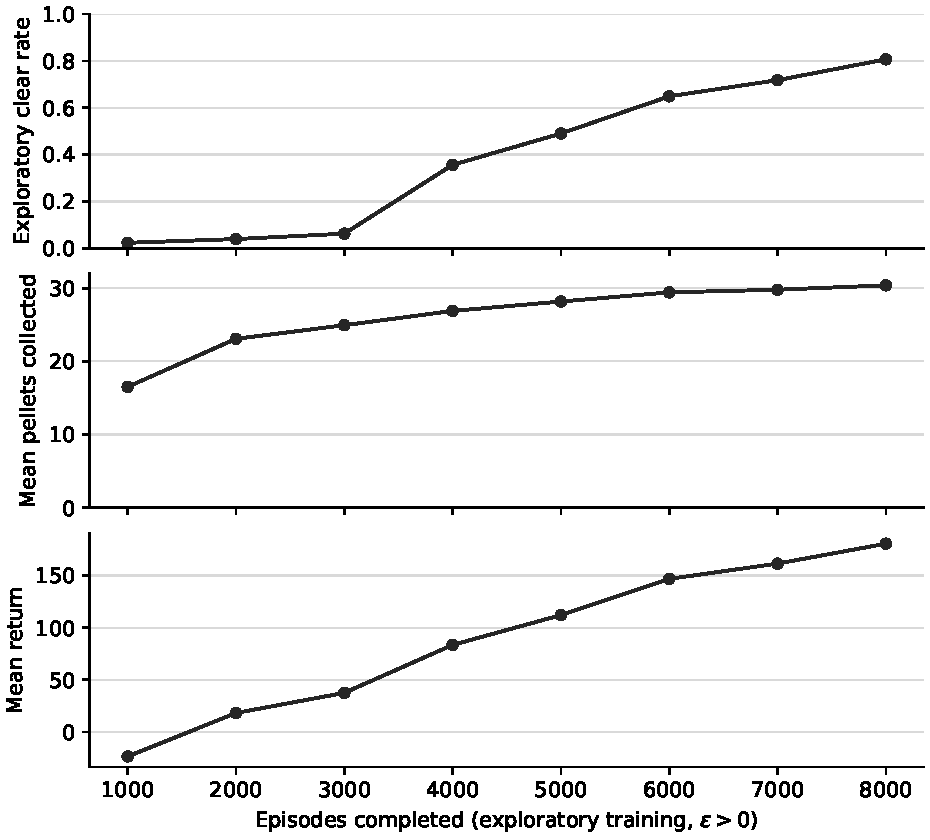
\includegraphics[width=0.88\linewidth]{figures/linear-sarsa-learning-curve.pdf}
  \caption{Exploratory training performance of linear True Online
    Sarsa($\lambda{=}0.5$). Each point is the mean over a 1{,}000-episode
    block on training seeds $0$--$7999$. Epsilon decays from 0.20 to 0.02, so
    these curves are not frozen greedy evaluation.}
  \label{fig:sarsa-learning-curve}
\end{figure}

\section{Implementation Audit and Reproducibility}

The final run followed several implementation corrections. Earlier checkpoints
were rejected after the project found that the step size did not account for
the number of active features, training ties used a fixed directional bias,
short diagnostic runs changed the epsilon-decay schedule, and the action mask
did not fully simulate Surge expiry and Orb pickup transitions. The final
implementation normalizes the step size by $\lVert x \rVert^2$, randomizes
training ties, decays epsilon over a fixed 8,000-episode horizon, and dry-runs
the next ten physics ticks for each valid-action check.

The project also validates deterministic game rules across TypeScript and
Python. The test suite includes 15 shared rule-parity fixtures, 90 Python unit
tests, and 15 TypeScript tests. The selected NPZ checkpoint exports exactly to
the tracked sparse browser JSON artifact: all 33,195 nonzero indices and
weights match.

\section{Discussion}

The results support the claim that linear value approximation is sufficient for
strong performance in this specific environment. Several conditions make that
possible. The state is structured numeric data rather than a high-dimensional
image. The feature map represents nearby collectibles, obstacles, enemy state,
and local mobility. The enemy follows deterministic dynamics. Finally, the
action mask removes directions that would collide during the next decision
interval.

The result should not be generalized to arbitrary games. It describes one
environment distribution, one selected hyperparameter configuration, and one
successful training run. The work nevertheless shows that a neural network is
not automatically necessary for a structured control task with a large
continuous observation representation.

\section{Limitations and Future Work}

\subsection{Priority 0: browser rollout parity}

The browser loads the exported model and matches Python on synthetic feature,
Q-value, and action tests. Full browser rollouts do not yet reproduce Python
evaluation exactly: TypeScript clears 93 of 100 evaluated seeds, whereas Python
clears 96. The browser queries the controller after a physics tick has reduced
the Surge timer, while Python presents the state at the decision boundary.
TypeScript also feeds double-precision values into the hash encoder whereas the
Python observation is float32. Future work should select the browser action
before clock mutation, round features through float32, and add an end-to-end
seeded Python--TypeScript rollout test.

\subsection{Priority 1: independent training runs and evaluation hygiene}

The study reports one training run with agent seed 73. A high score may partly
reflect a favorable optimization trajectory. The next scientific experiment
should train the selected configuration with five to ten independent agent
seeds, evaluate each frozen policy on the same validation environments, and
report the mean, spread, and worst-run performance.

Future model selection should use only validation environments. After choosing
the representation and hyperparameters, a new final seed range should be
evaluated once. This will avoid overlap between development evaluations and the
final reported benchmark.

\subsection{Priority 2: failure analysis and artifact provenance}

Aggregate clear rate does not identify why failures occur. Future experiments
should save capture and timeout trajectories and analyze enemy distance,
remaining pellets, Surge state, local action masks, Q-values, and arena
geometry near failure. The project should archive the NPZ checkpoint, JSONL
training log, evaluation JSON, command line, dependency versions, Git commit,
and model hash with each reported experiment.

\subsection{Priority 3: ablations, robustness, and model comparisons}

The next experiments should test the contribution of each design choice:
remove action-mask, bar, Orb, enemy-clock, and pellet-ranking features; vary
$\alpha$, $\lambda$, epsilon schedules, tile capacity, and tiling resolution;
and compare results on validation environments. Robustness tests should vary
enemy speed, starting positions, obstacle distributions, and enemy behavior.
Only after a fair validation comparison should the project compare the linear
agent with the planned neural Expected-Sarsa set encoder.

\section{Conclusion}

This work empirically demonstrates that a sparse, interpretable linear True
Online Sarsa($\lambda$) controller can achieve high greedy clear rates in the
Orbit Chase procedural environment. The result depends on the chosen state
representation, action mask, deterministic simulator, and evaluation protocol.
The next work should first make browser rollouts match Python exactly, then
measure stability across independent training runs and new evaluation
conditions.

\begin{thebibliography}{9}

\bibitem{sutton-barto-2018}
Richard S. Sutton and Andrew G. Barto.
\newblock \emph{Reinforcement Learning: An Introduction}.
\newblock Second edition, MIT Press, 2018.

\bibitem{van-seijen-2016}
Harm van Seijen, A. Rupam Mahmood, Patrick M. Pilarski, Marlos C. Machado, and
Richard S. Sutton.
\newblock True Online Temporal-Difference Learning.
\newblock \emph{Journal of Machine Learning Research}, 17(145):1--40, 2016.

\end{thebibliography}

\end{document}
